\section{Programstruktur}
Baseret på de førnævnte krav blev designfasen påbegyndt. Målet var at forsimple opgaven for brugeren så meget som overhoved muligt, da det ikke vil kunne forvæntes at denne person kender noget til det bagvedlæggende system. 
Tilsvarende ønskes der en simpel og generel anvendelse af programmets services fra de høje lag nær chat-klienten, hvor imod de mere administrative og praktiske funktionaliteter skal håndteres længere nede i systemet.

\begin{figure}[h!]
\centering
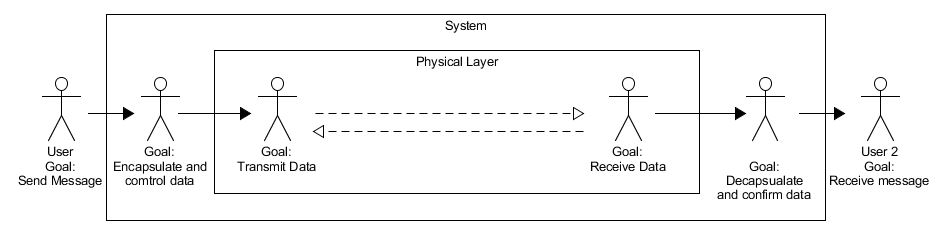
\includegraphics[scale=0.5]{Billeder/ProgramOpbygning1.JPG}
\caption{System opbygning - første udkast}
\label{fig:Blokdiagram}
\end{figure}

Figur \ref{fig:Blokdiagram} viser første udkast til programmets struktur i grove træk. Afsenderen modtager data fra brugeren, og indkapsler dette i en format modtageren er i stand til at bearbejde. Herfra tager det næste lag sig ad den reelle transmission og afkodning af informationen. Dette lag er upålideligt, så modtageren skal tilsvarende her validere indholdet og rækkefølgen af informationen får at kunne sikre at informationen når korrekt frem til brugeren. 

I og med at den ønskede applikation er et chat-program, er det af høj prioritet, at den logiske forbindelse mellem de to brugere er pålidelig. Dette indebære at det som afsenderen skriver skal være præcis det samme som modtageren læser. Systemet vil derfor tage udgangspunkt i TCP/IP, da denne protokol vigtigst af alt tilbyder en pålidelig overførsel af data. 


\subsection{Designklassediagram}
Næste step i arbejdsprocessen bliver at opsætte et klasse diagram, hvor i dataoverførelsen skal nedprydes i flere klasser med hver sit ansvarsområde, og funktionaliteter der passer hertil. Normalt kræver det, for at kunne udarbejde et systemklassediagram, at der inden er udarbejdet en domænemodel, med objekter fra den virkelige verden, men da dette projekt er et rent software problem, vil dette step ikke tilføre nogen værdi til projektet. 

\begin{figure}[h]
\centering
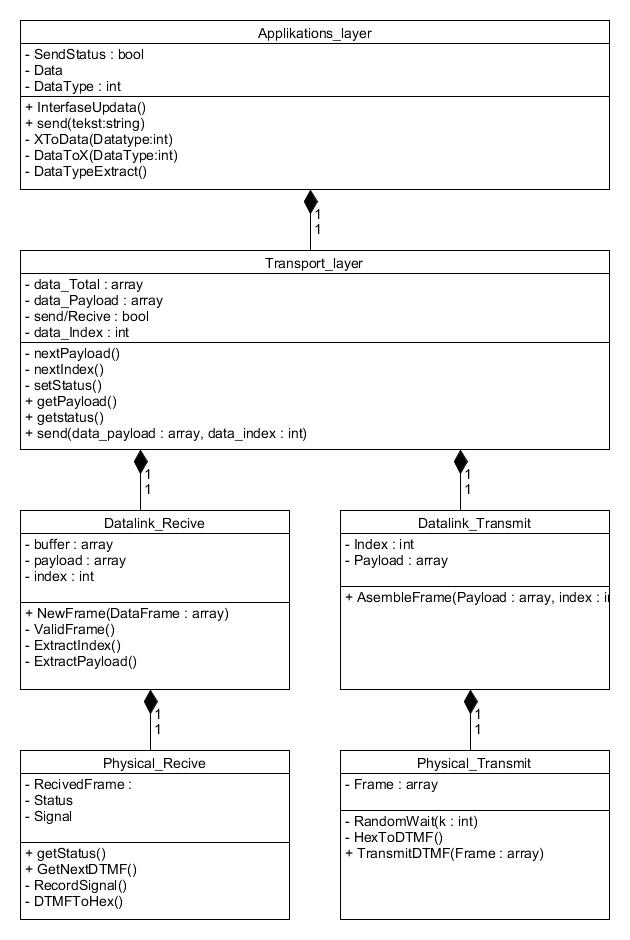
\includegraphics[scale=0.45]{Billeder/Klassediagram_v1.jpg}
\caption{Her vises systemklassediagram}
\label{fig:Klassediagram_v1}
\end{figure}

Det er ønsket at opnå en lagdelt struktur af programmet, da dette giver den fordel at ændringer på et lag ikke påvirker resten af programmets virkemåde, sålænge at inputtet og outputtet forbliver af samme format. Programmet er inddelt i fire lag:  Applikationslaget, transprotlaget, datalinklaget og det fysiske lag. Heraf er Datalinklaget og det fysiske lag opdelt i en afsender og modtager del. Dette ses af figur \ref{fig:Klassediagram_v1}. Denne struktur er inspireret af internettets syvlagsmodel, men da der ikke er behov for at route datapakker, vil der ikke være behov for netværkslaget. 

For at anvende af den service programmet tilbyder, er det nok at inkludere klassen "ApplicationLayer" og oprette et objekt heraf. Dette kan lade sig gøre de de underliggende objekter håndteres af applikationslaget. Applikationslaget kan derfor betragtes som værende systemets "controller". 

Det opstillede designklassediagram vil blive anvendt som en retningslinje for programmets opbygning, men da det i dette stadie af projektet kan være svært at tage højde for alt, vil det ikke være utænkeligt der måtte forkomme ændringer her i.


\subsection{Ansvarsfordeling til klasser}
Hvordan forvæntes de forskellige “sorte kasser” at arbejde sammen (grænse flader)

-Udpenslende forklaring af ansvarsfordeling og programstruktur.  

hvert lag får tildelt et ansvarsområde 
seberation of conserns

Derfor vil opgraderinger i konverteringen på applikationslaget være nok til at lade systemet understøtte flere datatyper (billeder, lyd og filer)